\documentclass[english,acmlarge,nonacm,natbib=false,urlbreakonhyphens=false,screen,11pt]{acmart}
\usepackage{babel}
\usepackage{csquotes}
\usepackage{listings}
\usepackage[style=alphabetic]{biblatex}
\geometry{
    a4paper,
    % vmargin=120pt,
    % hmargin=120pt,
}

\title{Reproducing Text Summarization with Pretrained Encoders}
\author{Jan Heinrich Reimer}
\orcid{0000-0003-1992-8696}
\affiliation{
    \institution{Martin Luther University Halle-Wittenberg}
    % \department{Institute for Computer Science}
    \streetaddress{Von-Seckendorff-Platz~1}
    \postcode{06108}
    \city{Halle (Saale)}
    % \state{Sachsen-Anhalt}
    \country{Germany}
}
\email{jan.reimer@student.uni-halle.de}

% Don't display a book title or conference.
\acmBooktitle{}
\acmConference{}{}{}

\addbibresource{../literature/literature.bib}
\nocite{*} % TODO Remove before publishing.


\newcommand{\todocite}{{\color{red}[TODO]}}

\begin{document}

\begin{abstract}
    Large pretrained transformer encoders like \Bert~\cite{DevlinCLT2019} have successfully been used for various tasks from the field of natural language processing~\cite{LiuL2019}. \citeauthor{LiuL2019} build upon the pretrained \Bert model to tackle extractive and abstractive text summarization~\cite{LiuL2019}. Their deep neural abstractive summarization model outmatches many previously state-of-the-art summarizers in informativeness and fluency measured using \Rouge metrics~\cite{LiuL2019,Lin2004}.
Since their publication, other fine-tuning models were introduced that surpass their performance~\cite{AghajanyanSGGZG2020,SavelievaAR2020}.
In this report, we reproduce the abstractive summarization experiments of~\citeauthor{LiuL2019} using the Flux~\cite{InnesSFGRJKPS2018} framework by re-implementing their \BertSumAbs model.
We highlight differences and difficulties in experimental replication to build a better understanding of abstractive summarization using pretrained encoders. 

\end{abstract}

\maketitle

\section{Introduction} % 50/300 points, 17%

The Web enables access to huge amounts of textual data, like news articles.
However, most web documents are unstructured and thus difficult to analyze.
For instance, it is hard to follow current news events, if we would have to read each article entirely.
Text summarization in general can be used to condense larger texts to its essential contents~\cite[xix]{Torres-Moreno2014}.
Often software is used for automatic text summarization and in recent years
automatic text summarization has become an important problem in natural language processing for information retrieval~\cite[xxi]{Torres-Moreno2014}, often tackled by deep neural networks~\cite{CelikyilmazBHC2018,LiuL2019,NallapatiZSGX2016,PaulusXS2018,SeeLM2017}.
The task of text summarization can be divided into two main approaces: extractive and abstractive summarization. In extractive text summarization, the task is to extract most important sentences from the source text. In abstractive text summarization new text is generated which does not necessarily have to match sequences of the source~\cite[28]{Torres-Moreno2014} nor its vocabulary~\cite{NallapatiZSGX2016}.
Particularily, abstractive summaries generated automatically aim to be more comparable to summaries prouced by human~\cite[220]{Torres-Moreno2014}.

Previous neural approaches to abstractive summarization are based on sequence-to-sequence modelling~\cite{NallapatiZSGX2016}, pointing to the source text~\cite{SeeLM2017}, or communicating agents~\cite{CelikyilmazBHC2018}.
Though, the limited amount of training data in benchmark datasets suited for abstractive summarization makes it difficult to train deeper neural networks.
For example, the articles from the \CnnDailyMail datasets contain only 242M~words of text, that could be used for training an abstraction model~\cite{HermannKGEKSB2015}.
With the availability of large pretrained language models like \Elmo~\cite{PetersNIGCLZ2018} and \Bert~\cite{DevlinCLT2019} it is often more efficient to fine-tune a pretrained language model, that already encodes semantics of a language~\cite{LiuL2019}.
The \Bert model, for instance, was trained on 3300M~words~\cite{DevlinCLT2019}, more than 10~times the training data available from the \CnnDailyMail datasets.
Apart from the advantages of higher amounts of training data, a pretrained language model could also potentially reduce learning cost, as models building upon a pretrained model only have to be fine-tuned, not trained from scratch~\cite{DevlinCLT2019}.

\citeauthor{LiuL2019} propose two new approaches to text summarization that leverage a pretrained \Bert model: a sentence classification architecture for extractive summarization~(\BertSumExt) and an encoder-deoder framework for abstractive summarization~(\BertSumAbs)~\cite{LiuL2019}.
In both tasks, the source text is encoded with pretrained \Bert transformers. Then for extractive summarization, sentence sequences from the \Bert encoder are again transformed and then classified whether they should be included in the summary.
For abstractive summarization, \Bert output embeddings are decoded using a transformer decoder and a linear layer is used to map embeddings back to the input vocabulary~\cite{LiuL2019}. In both cases, the \Bert encoder is jointly fine-tuned with input emeddings, classfier and/or decoder layers.
Notably, the abstractive summarization model, which we reproduce in this report,
follows an architecture very similar to neural machine translation and a neural machine translation toolkit is used in many parts of the \BertSumAbs implementation~\cite{LiuL2019,KleinKDSR2017}.

From the models proposed by \citeauthor{LiuL2019}, we choose the \BertSumAbs abstractive summarization model for our replication due to its promising trade-off between model complexity and performance in terms of \Rouge metrics on the \CnnDailyMail datasets~\cite{LiuL2019,HermannKGEKSB2015}.
Compared to previous neural approaches~\cite{SeeLM2017,PaulusXS2018}, it does not need copy nor coverage~\cite{LiuL2019}
Furthermore, the abstractive model also allows for more variation of the model's hyperparameters, e.g. changing the depth or width of the decoder's transformer layers. 
Even though the extractive model \BertSumExt outperforms previous approaches more  distinctly, it requires more complex preprocessing of input articles and the model changes aspects of \Bert's internals~\cite{LiuL2019}, requiring a separate, more detailed replication study.

\citeauthor{LiuL2019} claim that the \BertSumAbs model outperforms many previous state-of-the-art summarizers in informativeness and fluency, measured using the \RougeN{1}, \RougeN{2}, and \RougeL metrics~\cite{LiuL2019,Lin2004}.
We expect similar scores with our re-implemented model, but due to the lack of hardware resources for training such a big neural model we are unable to compare final \Rouge scores.
With our more idiomatic re-implementation we facilitate more in-depth analyzes of the \BertSumAbs and \TransformerAbs models by \citeauthor{LiuL2019}.
The technical difficulties we faced in training the \BertSumAbs model questions the usefullness of very large, pretrained encoder models like \Bert for abstractive text summarization, at least on a smaller budget. It remains an open question whether smaller variants like \BertTiny could achieve comparable \Rouge scores for abstractive summarization~\cite{TurcCLT2019}.

\section{Related Work} % 80/300 points, 27%

In the reproduced article, \citeauthor{LiuL2019} use the encoder from the pretrained \Bert language model to build absractive text summarization model~\cite{LiuL2019,DevlinCLT2019}.
While neural architectures have previously been used for abstractive summarization~\cite{NallapatiZSGX2016,SeeLM2017,Paulus2018}, it has been difficult to generate fluent yet informative summaries because those models can only model linguistics from limited training data~\todocite. Common benchmark datasets like the CNN/Daily Mail datasets for supervised learning contain far less data then the amount available for unsupervised pretraining of language models~\cite{HermannKGEKSB2015,DevlinCLT2019}.
By fine-tuning a transformer encoder-decoder architecture with pretrained encoders~\cite{VaswaniSPUJGKP2017,DevlinCLT2019}, \citeauthor{LiuL2019} leverage broader linguistic knowledge from the pretrained language model for generating better summaries~\cite{LiuL2019}.
As predicted in their article, now \todo{larger} language models are able to generate even better abstractive summaries~\todocite\cite{LiuL2019}.

\subsection{Abstractive Summarization}

\todo{What is abstractive summarization?}

% Reproduced approach is based on:
\citeauthor{Sutskever2014?,Chopra2016?,NallapatiZSGX2016}: neural encoder-decoder network as RNN.
\citeauthor{NallapatiZSGX2016}: sequence-to-sequence modelling, first to use CNN/Daily Mail~\cite{HermannKGEKSB2015} for evaluating summarization quality~\cite{T5}, generator/pointer setting.
\citeauthor{???}: abstractive summarization is a generative task similar to neural machine translation.

% Other approaches:
\citeauthor{Paulus2018,SeeLM2017}: generative models sometimes produce unnatural, repetitive summaries.
\citeauthor{Paulus2018}: attention over input and generated output, take into account what has already been generated (\Bert does that too with output transformers~\cite{DevlinCLT2019}?), uses teacher forcing.
\citeauthor{SeeLM2017}: hybrid pointer-generator network with coverage to avoid repetition and factual errors.

\subsection{Summarization With Pretrained Language Models}

% Reproduced approach is based on:
\citeauthor{DevlinCLT2019}: pretrained language model, based on multi-head attention~\cite{VaswaniSPUJGKP2017}, trained on a large corpus (3300M tokens), \Bert parameters jointly fine-tuned with task-specific parameters.
\citeauthor{Edunov2019?,Rothe2019?}: use \Bert for generative tasks.

% Reproduced approach:
\citeauthor{LiuL2019}: abstractive summarization as encoder-decoder generative approach, using pretrained \Bert encoder~\cite{DevlinCLT2019}, transformer decoder~\cite{VaswaniSPUJGKP2017}, custom trained position embeddings.
Open details not covered completely in the replicated article.
Which details can be explained and added by our reproduction.
Explain those particular details.
Which principles, ideas, or assumptions are used or made in the replicated approach?

% Other approaches:
\citeauthor{???}: other (larger) pretrained models used for abstractive summarization.
BART, BART+R3F, ERNIE-GENLARGE?

\section{Experimental Evaluation} % 70/300 points, 23%

We fine-tune and evaluate the \BertSumAbs summarization model from the reproduced paper by \citeauthor{LiuL2019} on a A100 GPU using the Flux framework on Julia~\cite{InnesSFGRJKPS2018,BezansonEKS2017,LiuL2019}.
A scaled-down variant of their \TransformerAbs model, that we call \TransformerAbsTiny, is trained from scratch on a GeForce MX150 GPU for testing our evaluation workflow.
We train both models using the CNN/Daily Mail datasets, but use the preprocessed variant by \citeauthor{LiuL2019} instead of the original data by \citeauthor{HermannKGEKSB2015}~\cite{LiuL2019,HermannKGEKSB2015}.
Our implementation resembles the same encoder-decoder architecture as used by \citeauthor{LiuL2019} and uses the same \BertBase model as the pretrained encoder~\cite{LiuL2019,DevlinCLT2019}.
Though, we do not tune any hyperparameters of either the model or the optimizers.
We also reimplement the beam search algorithm from scratch.
Due to instabilities in fine-tuning and hardware constraints we were unable to train the model for the full 200\,000 steps proposed by \citeauthor{LiuL2019}.
We assume that the complex hyperparameter settings and large model size used in their paper are prone to fine-tuning issues like we experienced, a problem that has recently gained more attention~\cite{DodgeISFHS2020
,ZhangWKWA2020,AghajanyanSGGZG2020}.


Describe implementation structure/approach. (Julia/Flux, , tokenization (\Bert), model structure (encoder-decoder, beam search), hyperparameter tuning, optimizer)

\subsection{Dataset}

We train and evaluate the summarization model on the CNN / Daily Mail dataset~\cite{HermannKGEKSB2015}, but use preprocessed data released by \citeauthor{LiuL2019} along with the replicated paper.
Our implementation is designed to automatically download both the pretrained \BertBase model and the preprocessed CNN/Daily Mail datasets from the Web, no manual downloads are needed.
From the preprocessed data we extract the source article and the target summary as raw text, join sentences to normalize separators, and tokenize with \Bert's word piece tokenizer~\cite{DevlinCLT2019}.

Describe raw data format.

Describe data preprocessing. (Pre-processed dataset from \citeauthor{LiuL2019}: Sentence splitting  with Stanford CoreNLP, entities are not anonymized.)

\subsection{Abstractive Summarizaion Model}

Transformer with 6 layers, 768 hidden units, hidden size of 2048.
Train for 200\,000 steps, snapshots every 2500 steps, gradient accumulation at every step.
Choose the single best snapshot for evaluation.

Describe simple tests/examples for checking implementation correctness. (Untrained model produces nonsense summaries.)

Describe implementation memory usage, complexity, and run time performance.
The full \BertSumAbs model contains 182M trainable parameters: 27M for embeddings, 85M for the encoder's transformer layers, 47M for the decoder's transformer layers, and 23M for the generator layer.

\subsection{Fine-tuning the pretrained model}

Describe training schedule.
Two Adam optimizers with~\(\beta_1 = 0.9\) and~\(\beta_2 = 0.999\).
Learning rates:
\begin{align}
    \eta_E &= 2e^{-3} \cdot \min( \text{step}^{-0.5},\ \text{step} \cdot 20\,000^{-1.5} ) \\
    \eta_D &= 0.1 \cdot \min( \text{step}^{-0.5},\ \text{step} \cdot 10\,000^{-1.5} )
\end{align}

Presumably because of the high number of parameters to tune, training this \BertSumAbs model on a A100 GPU uses about 40GB of memory at a speed of about 9 steps per minute.
Because of the slow training speed even on a powerful GPU we had to cancel training the model after 22\,500 steps.

\subsection{Beam Search}

\subsection{Experiments}

Describe experiment reproductions.

\paragraph{Training Loss}

\begin{figure}
    \centering
    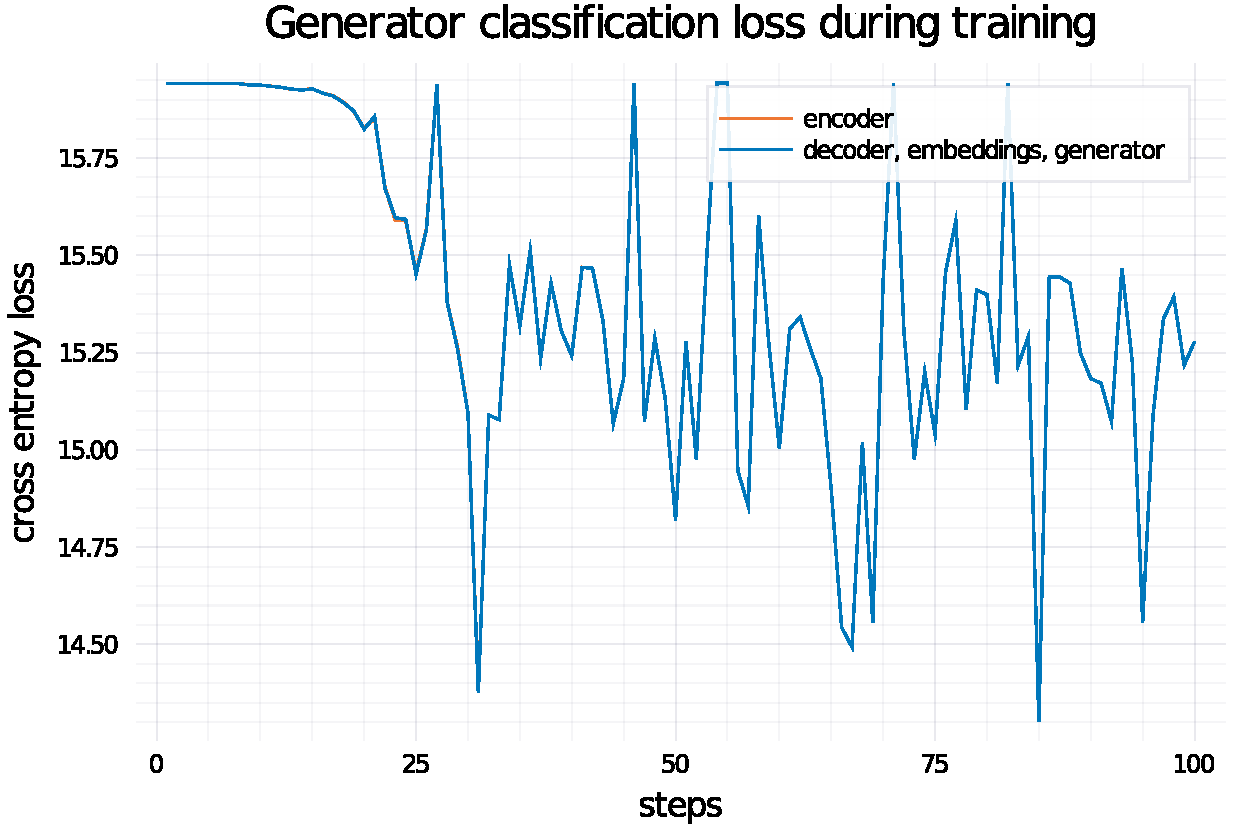
\includegraphics[width=0.7\linewidth]{training-loss-bert-abs-100.pdf}
    \caption{Cross entropy between predicted token probabilities and ground truth labels for the first 100 training steps of training the \BertSumAbs model.}
    \label{training-loss-bert-abs}
\end{figure}

\begin{figure}
    \centering
    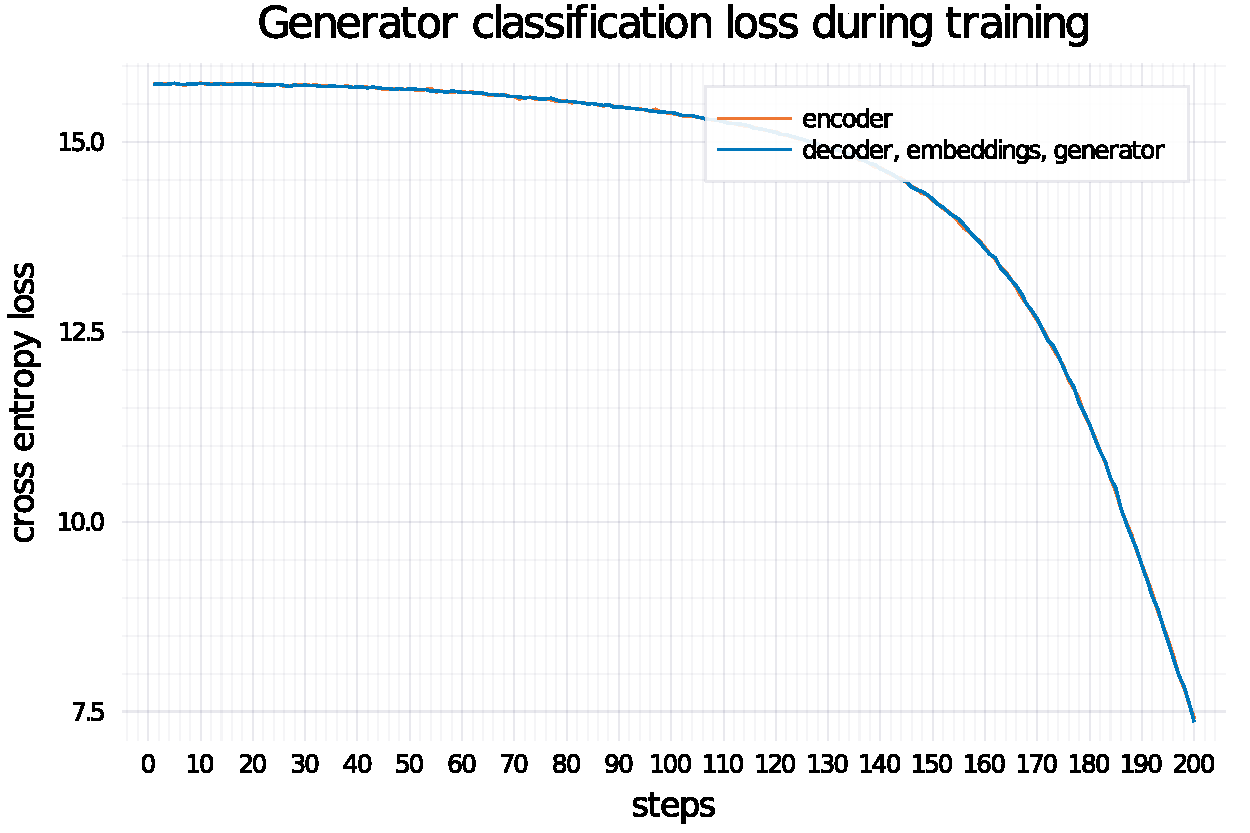
\includegraphics[width=0.7\linewidth]{training-loss-transformer-abs-tiny.pdf}
    \caption{Cross entropy between predicted token probabilities and ground truth labels for the first 200 training steps of training the \TransformerAbsTiny model.}
    \label{training-loss-transformer-abs}
\end{figure}


\paragraph{Summary Quality}

Describe \Rouge scores for some examples.

Describe/list difficulties or problems. (Pretrained data not available from a data source that allows automatic downloads.)

\section{Conclusion and Future Work} % 30/300 points, 10%

Is the chosen approach good enough to consider the problem solved?
Which difficulties in the original approach did arise during reproducing the experiments?

\subsection{Future Work}

Which fields do we consider relevant/important for future research?

Use smaller \Bert model, e.g. \BertTiny. Can that be trained with less resources? Does it generate good summaries?

Tune hyperparameters for the transformer decoder, an evaluation that is missing from the replicated paper.

\appendix
\section{Appendix (70/300)}

\subsection{Git History}

\subsection{Implementation}

\paragraph{Data Pre-processing}

\paragraph{Model}

\paragraph{Tests, Output, Plots}
Tests, Output, Plots for demonstrating workflow and correctness.

\paragraph{Open Details}
Evaluation of Open Details in the replicated article.

\paragraph{Replicated Experiments}
Describe experiment and evaluation implementation.

\paragraph{Evaluation}


\printbibliography

\end{document}